\documentclass[fleqn]{article}

\usepackage{polski}
\usepackage[utf8]{inputenc}
\usepackage[polish]{babel}
\usepackage{parskip}
\usepackage{icomma}
\usepackage[a4paper,includeheadfoot,margin=2.54cm]{geometry}
\usepackage{float}
\usepackage{graphicx}
\usepackage{amsmath}
\usepackage[hypcap=true]{subcaption}
\usepackage{xcolor}
\usepackage{transparent}
\usepackage{listings}
\usepackage[colorlinks=true, linkcolor=blue, pdfborder={0 0 0}]{hyperref}

\renewcommand\thesection{\arabic{section}.}
\renewcommand\thesubsection{\alph{subsection})}
\renewcommand\thesubsubsection{}
\newcommand\square[1]{
	\fcolorbox{black}{#1}{\rule{0pt}{6pt}\rule{6pt}{0pt}}
}

\brokenpenalty=1000
\clubpenalty=1000
\widowpenalty=1000

\title{TM -- Laboratorium 1.}
\author{Krystian Chachuła \\ Dawid Gruszczyński \\ Marcin Skrzypkowski}

\begin{document}

\maketitle

\setcounter{page}{0}
\thispagestyle{empty}

\pagebreak

\setcounter{page}{1}

\section{Wstęp}

Na pierwszym laboratorium mieliśmy za zadanie oswoić się z układem FPGA symulującym mikroprocesor Z80 przez rozpoznanie podstawowych instrukcji wejścia/wyjścia oraz pamięci. Ćwiczenie składało się z trzech punktów: przedstawienia podstawowych instrukcji na oscyloskopie, zaprojektowania i skonstruowania układu aktywującego sygnał $\overline{WAIT}$ na zadaną ilość taktów po spełnieniu określonych warunków oraz zbudowania układu pułapkującego procesor do czasu wyzwolenia przełącznikiem bistabilnym.

Zaprojektowane przed laboratorium układy zbudowaliśmy z dostępnych układów SML-3:

\begin{itemize}
	\item \textbf{10\_PS1} (moduł zasilacza)
	\item \textbf{100\_LED8} (zestaw 8 diod)
	\item \textbf{13x\_IN6} (zestaw bistabilnych przełączników)
	\item \textbf{202\_NAND} (zestaw bramek \textit{NAND})
	\item \textbf{380\_NOTx6} (moduł sześciu bramek negujących)
	\item \textbf{451\_IN\_4xHEX} (zestaw przełączników szesnastkowych)
	\item \textbf{331\_MUX-Dx2} (zestaw multiplekserów oraz przerzutników typu D)
	\item \textbf{400\_74194x2} (moduł rejestrów przesuwnych)
	\item procesor Z80 zrealizowany w układzie FPGA
\end{itemize}

Schematy do zadania drugiego i trzeciego podane są podczas omawiania poszczególnych problemów. Programy pisane w Assembly dla procesora Z80 wgrywaliśmy z pomocą aplikacji NoICE, która umożliwiała sprawdzenie adresów i wielkości poszczególnych instrukcji oraz testowanie ich i uniknięcie nieskończonej pętli podczas testowania programu, od której jedyną ucieczką był reset procesora. Aby jednak uzyskać wyraźny obraz na oscyloskopie, należało przełączyć aplikację w tryb RUN, gdyż w przeciwnym wypadku oscylogram pokazywał również polecenia wysyłane przez sam program NoICE, co uniemożliwiało analizę naszego programu.

\section{Odczytywanie przebiegów instrukcji na oscyloskopie}

Pierwsze zadanie polegało na obserwacji i opisie pięciu przebiegów sygnałów procesora: wczytywanie i zapis do pamięci, wczytywanie i zapis do przestrzeni wejścia/wyjścia oraz cykl pobierania kodu instrukcji.
W celu realizacji zadania napisaliśmy prosty program w Assembly Z80, który po uruchomieniu w aplikacji NoICE i włączeniu trybu RUN pozwalał na obserwację wyżej wymienionych przebiegów.

\lstinputlisting{src/1.lst}

\begin{figure}[H]
	\centering
	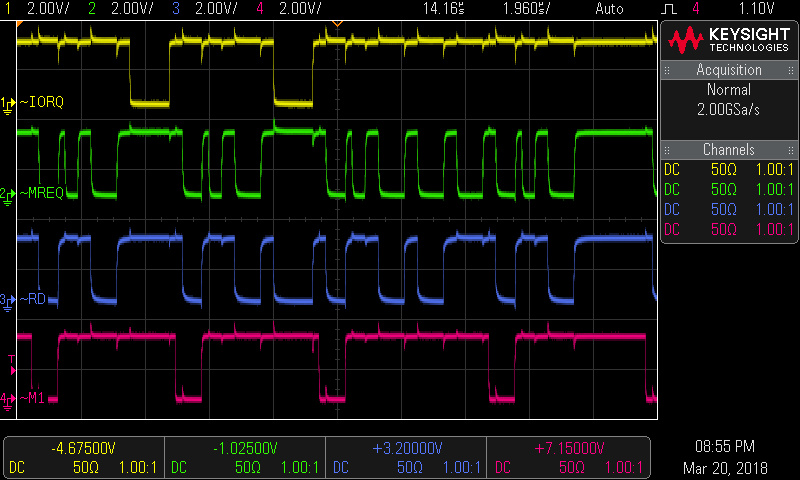
\includegraphics[width=0.72\textwidth]{img/1a.png}
	\caption{Sygnały sterujące szyną (jeden przebieg pętli)}
	\label{fig:1a}
\end{figure}

\subsection{Cykl fetch}

Na początku realizacji każdego polecenia mikroprocesor pobiera kod instrukcji, co jest sygnalizowane stanem niskim na wyjściach $\overline{MREQ}$, $\overline{RD}$ oraz $\overline{M1}$. Zaraz potem następuje odświeżenie pamięci sygnalizowane stanem niskim jedynie na wyjściu $\overline{MREQ}$ (oraz $\overline{RFSH}$, lecz nie widać tego na oscylogramie). W trakcie odświeżania dekodowany jest także kod pobranej instrukcji.
Cały cykl można zaobserwować w bloku \square{red} na rysunku \ref{fig:1a}. Nieprzedłużony sygnałem $\overline{WAIT}$ trwa 4 cykle zegarowe.

\subsection{Cykl odczytu z pamięci}

Podczas tego cyklu zaznaczonego w bloku \square{cyan} następuje pobranie argumentu operacji z pamięci.
Sygnalizowane jest to niskim stanem na wyjściach $\overline{MREQ}$ i $\overline{RD}$. Jej wykonanie trwa zwykle 3 cykle zegarowe.
%TODO: sprawwdzić jakie to polecenie

\subsection{Cykl zapisu do układów wejścia/wyjścia}

Cykl zapisu do pamięci:
Podczas cyklu \square{yellow} następuje zapis do pamięci realizowany przez instrukcję LD, sygnalizowane jest to stanem niskim na wyjściach $\overline{MREQ}$ i $\overline{WR}$ ($\overline{WR}$ nie jest widoczne na oscylogramie). Sygnał $\overline{WR}$ pojawia się na wyjściu procesora jeden cykl zegarowy po wystawieniu sygnału $\overline{MREQ}$, by dane na szynie zdążyły się ustabilizować. Cała instrukcja zapisu trwa zwykle 3 cykle zegarowe.

\subsection{Cykl odczytu z przestrzeni wejścia/wyjścia}

Podczas cyklu zaznaczonego w bloku \square{violet} następuje odczyt z układów wejścia/wyjścia realizowany przez instrukcję IN, sygnalizowany jest stanem niskim na wyjściach $\overline{IORQ}$ i $\overline{RD}$. Podczas wykonywania instrukcji z przestrzeni wejścia/wyjścia automatycznie jest wstawiany jeden cykl $\overline{WAIT}$. Jest to spowodowane późnym uaktywnieniem sygnału $\overline{IORQ}$ (jest aktywowany w drugim cyklu zegarowym), co uniemożliwia wolniejszym układom zewnętrznym na wystarczająco szybką reakcję i uaktywnienie przez nie sygnału $\overline{WAIT}$ w tym samym cyklu zegarowym tak, by został on wykryty przez mikroprocesor. Z tego powodu ta instrukcja trwa zwykle 4 cykle zegarowe.

\subsection{Cykl zapisu do pamięci}

Podczas cyklu zaznaczonego w bloku \square{green} następuje zapis do pamięci realizowany przez instrukcję LD, sygnalizowane jest to stanem niskim na wyjściach $\overline{MREQ}$ i $\overline{WR}$ ($\overline{WR}$ nie jest widoczne na oscylogramie). Również w tej instrukcji dodawany jest automatycznie sygnał $\overline{WAIT}$, dlatego cykl zapisu w przestrzeni wejścia/wyjścia trwa zwykle 4 cykle zegarowe.

Z powyższego kodu można również wyczytać wielkości poszczególnych poleceń. instrukcja OUT ma jeden bajt kodu instrukcji oraz jeden bajt pobranego argumentu 0h, polecenie IN podczas instrukcji fetch również pobiera jeden bajt i jeden bajt argumentu 0h, natomiast polecenie LD pobiera jeden bajt kodu instrukcji i jeden dwubajtowy argument, (najpierw mniej, następnie bardziej znaczące bity adresu 1900h). Polecenie JR poza kodem instrukcji pobiera dodatkowo jeden bajt służący do obliczenia relatywnego skoku.

\section{Generowanie sygnału opóźniającego}

Naszym zdaniem było wstawianie \textbf{dwóch} dodatkowych taktów opóźnienia po wykryciu \textbf{odczytu danych z przestrzeni wejścia/wyjścia}. Procesor automatycznie wstawia jeden takt opóźnienia przy wykonywaniu instrukcji dotyczących tej przestrzeni, zatem łącznie mieliśmy uzyskać trzy takty opóźnienia.

Pierwszą naszą czynnością było stworzenie funkcji logicznej, która przyjmowała wartość $\textbf{1}$, gdy był spełniony warunek z treści zadania i $\textbf{0}$ w przeciwnym przypadku. Następnie zaprojektowaliśmy układ kombinacyjny realizujący tę funkcję. Początkowo wykorzystaliśmy bramki \textit{NAND} oraz \textit{NOT}, ale ze względu na trudność modyfikacji oraz małą przejrzystość takiego układu finalnie zdecydowaliśmy się na wykorzystanie multipleksera.

\begin{figure}[H]
	\centering
	\begin{subfigure}[b]{0.8\textwidth}
		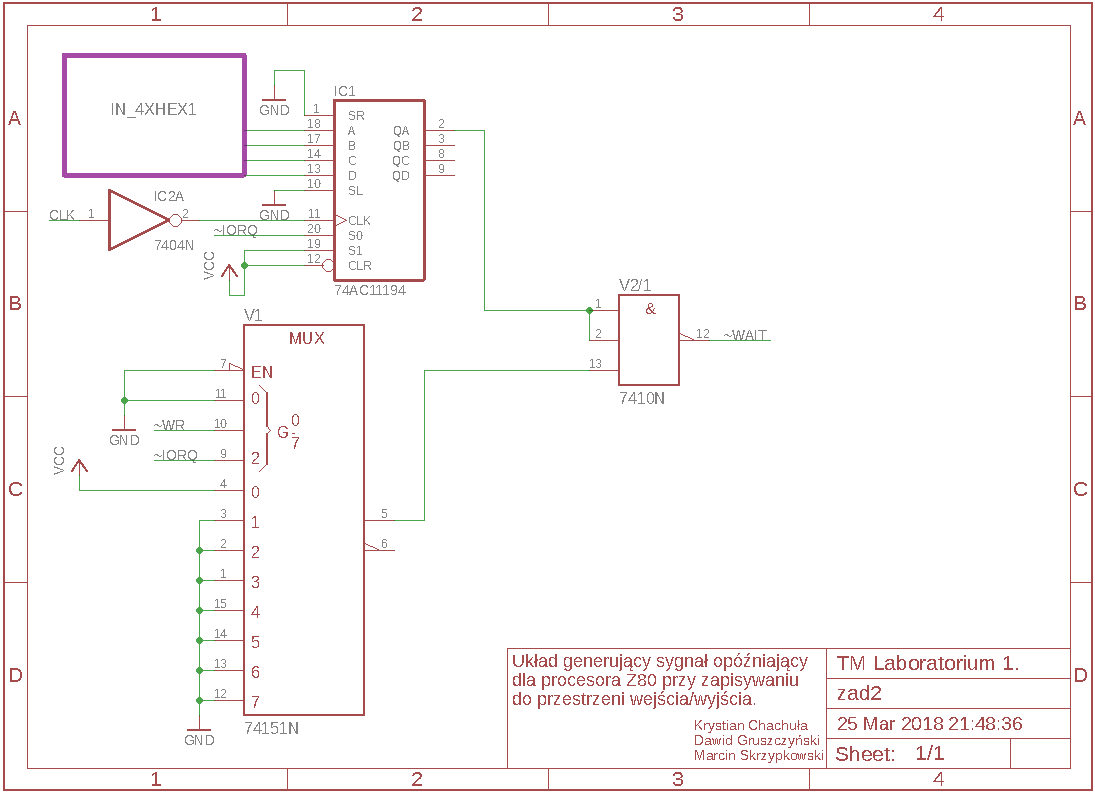
\includegraphics[width=\textwidth]{img/z2.png}
	\end{subfigure}
	\caption{Schemat elektryczny układu będącego rozwiązaniem zadania drugiego}
	\label{fig:z2}
\end{figure}

Do odliczania taktów zegara procesora zdecydowaliśmy się użyć rejestru przesuwnego z modułu SML-3 \textbf{400\_74194x2}. Pozwala on zliczyć maksymalnie 4 takty zegara, więc biorąc pod uwagę wbudowany takt oczekiwania byliśmy w stanie dodać maksymalnie 3 takty. Było to jednak wystarczające do wykonania zadania. Wejściem taktującym rejestru był zanegowany sygnał zegarowy procesora, ponieważ sygnał $\overline{WAIT}$ był próbkowany przez procesor podczas opadającego zbocza zegara, więc każde przesunięcie zawartości rejestru oznaczało wydłużenie sygnału opóźniającego o jeden takt. Alternatywą do naszego rozwiązania było użycie licznika, lecz rejestr był rozwiązaniem prostszym.

Ładowanie rejestru oraz przesuwanie odbywało się poprzez podłączenie do wejścia $S0$ sygnału $\overline{IORQ}$: w stanie wysokim następowało ładowanie rejestru, a w stanie niskim przesuwanie.

Ilość wymaganych przez zadanie taktów zegara była ładowana do rejestru z modułu przełączników szesnastkowych ${IN\_4xHEX}$. Ilość taktów była równoważna z ilością kolejnych jedynek w rejestrze patrząc od najmniej znaczącego bitu. Umożliwiło to późniejszą trywialną modyfikację zadania, gdy mieliśmy wprowadzić przykładowo jeden dodatkowy tak oczekiwania. Liczba ładowana z przełączników była już uzupełniona o takt automatyczny, więc gdy ładowaliśmy do rejestru liczbę $3_{10} = 11_2$, oznaczało to wprowadzenie dwóch taktów oczekiwania, z czego jeden był automatyczny. Uzyskiwaliśmy więc przedłużenie o jeden takt zegarowy.

Wyjście multipleksera oraz najmniej znaczący bit rejestru zostały doprowadzone do wejść bramki \textit{NAND}. W ten sposób otrzymaliśmy wymagany sygnał $\overline{WAIT}$.

Podczas testowania złożonego układu korzystaliśmy z programu z punktu 2.  W kolorze \square{blue} widać funkcję $\overline{WAIT}$ generowaną przez nasz układ. Dla położenia 0 i 1 przełącznika szesnastkowego sygnały $\overline{IORQ}$ oraz $\overline{RD}$ nie ulegają wydłużeniu. Powodem jest pokrywanie się pierwszego wygenerowanego taktu oczekiwania z tym wbudowanym, wstawianym przez procesor. Dlatego też widoczna na oscylogramach \ref{fig:2a} i \ref{fig:2b} instrukcja odczytu z przestrzeni wejścia/wyjścia w obu przypadkach trwa 4 takty zegara. Na wykresach \ref{fig:2c}, \ref{fig:2d} i \ref{fig:2e} wyraźnie widać, że została przedłużona kolejno o jeden, dwa oraz trzy takty zegarowe. Poniżej znajduje się schemat funkcji generującej takty oczekiwania oraz przebiegi sygnałów dla ustawień przełącznika szesnastkowego 0, 1, 3, 7, 15 (wykresy kolejno \ref{fig:2a}, \ref{fig:2b}, \ref{fig:2c}, \ref{fig:2d} oraz \ref{fig:2d}).

\begin{figure}[H]
	\centering
	\begin{subfigure}[b]{0.49\textwidth}
		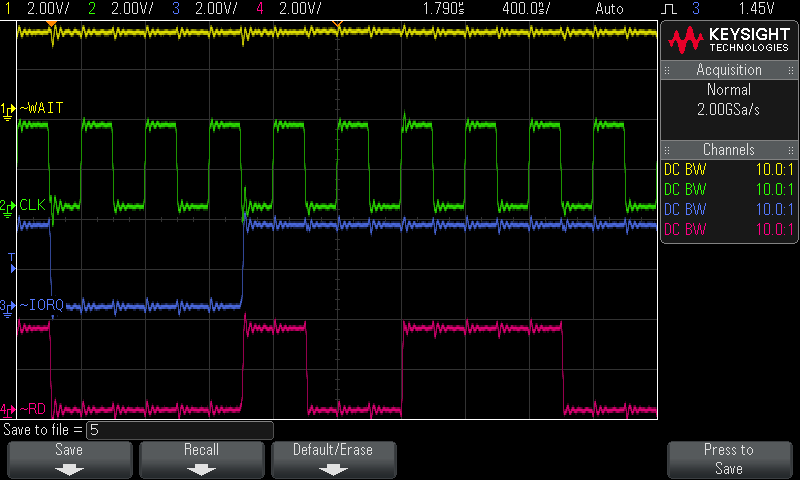
\includegraphics[width=\textwidth]{img/2a.png}
		\caption{0 wygenerowanych t. opóźnienia (efektywnie 1)}
		\label{fig:2a}
	\end{subfigure}
	\begin{subfigure}[b]{0.49\textwidth}
		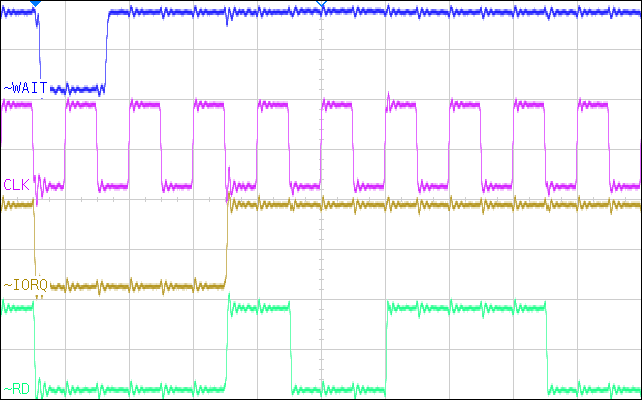
\includegraphics[width=\textwidth]{img/2b.png}
		\caption{1 wygenerowany t. opóźnienia (efektywnie 1)}
		\label{fig:2b}
	\end{subfigure}
	\centering
	\begin{subfigure}[b]{0.49\textwidth}
		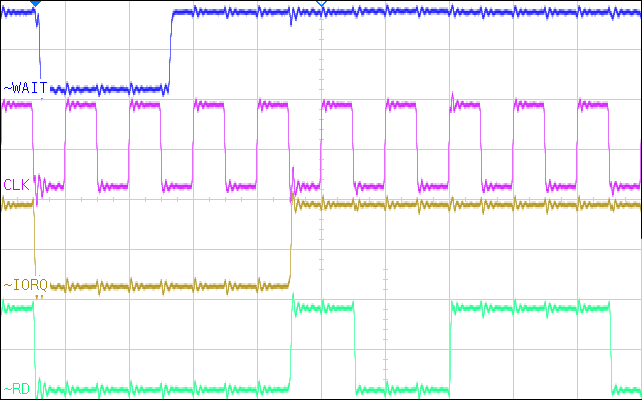
\includegraphics[width=\textwidth]{img/2c.png}
		\caption{2 wygenerowane takty opóźnienia}
		\label{fig:2c}
	\end{subfigure}
	\begin{subfigure}[b]{0.49\textwidth}
		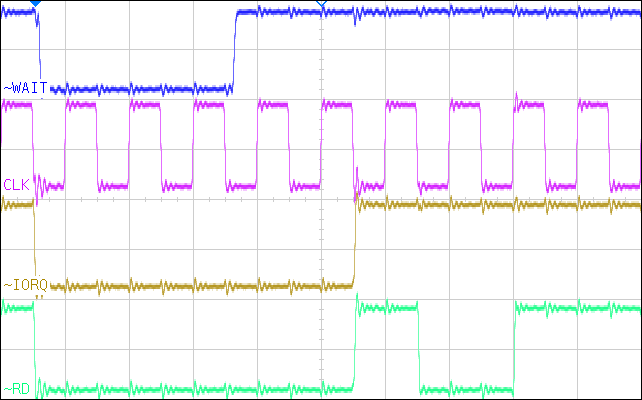
\includegraphics[width=\textwidth]{img/2d.png}
		\caption{3 wygenerowane takty opóźnienia}
		\label{fig:2d}
	\end{subfigure}
	\begin{subfigure}[b]{0.49\textwidth}
		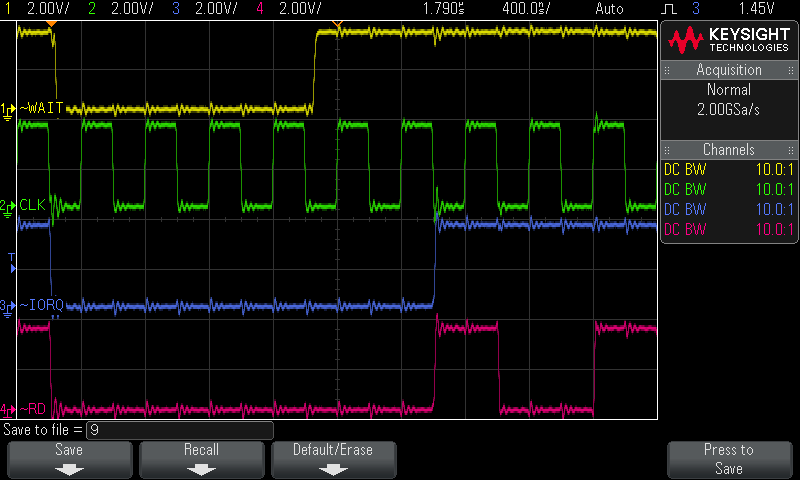
\includegraphics[width=\textwidth]{img/2e.png}
		\caption{4 wygenerowane takty opóźnienia}
		\label{fig:2e}
	\end{subfigure}
	\begin{subfigure}[b]{0.49\textwidth}
	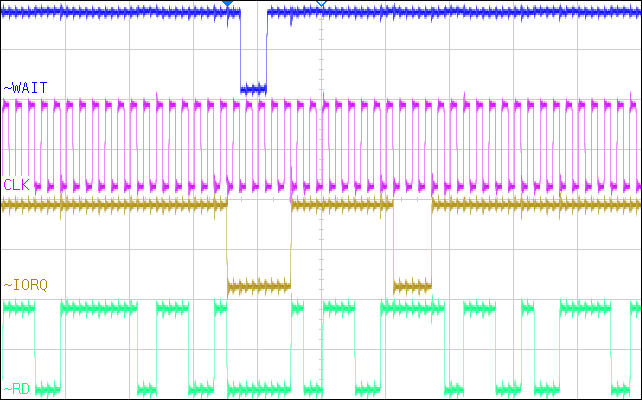
\includegraphics[width=\textwidth]{img/2f.png}
	\caption{3 takty opóźnienia (szeroka perspektywa)}
	\label{fig:2f}
\end{subfigure}
	\caption{Sygnały manipulujące szyną danych przy różnych ustawieniach układu opóźniającego}
	\label{fig:2}
\end{figure}

\pagebreak

\section{Wstrzymywanie pracy procesora}

Ostatnim zadaniem była modyfikacja poprzedniego układu w taki sposób, aby zamiast wstawiać takty oczekiwania, generować sygnał $\overline{WAIT}$ do momentu uzyskania zbocza przełącznika.
Zdecydowaliśmy się zastąpić rejestr przerzutnikiem typu D, gdyż element zliczający nie był już potrzebny, a wystarczył prosty układ z pamięcią. Przerzutnik pozwalał nam też na wykrywanie zbocza przełącznika przez podłączenie go do wejścia zegarowego.
W normalnych warunkach (gdy procesor nie wpadał w pułapkę) przerzutnik był resetowany sygnałem $M1$ (na wyjściu $\overline{Q}$ pojawiał się sygnał $\textbf{1}$, oznaczający gotowość do zatrzymania procesora). Do wejścia D podpięty był stały sygnał wysoki, dzięki czemu zbocze przełącznika powodowało dezaktywację sygnału $\overline{WAIT}$ poprzez resetowanie wyjścia $\overline{Q}$ przerzutnika. Do wejścia $\overline{SET}$ przerzutnika był na stałe podłączony sygnał $\textbf{1}$, gdyż nie było potrzeby z niego korzystać.

\begin{figure}[H]
	\centering
	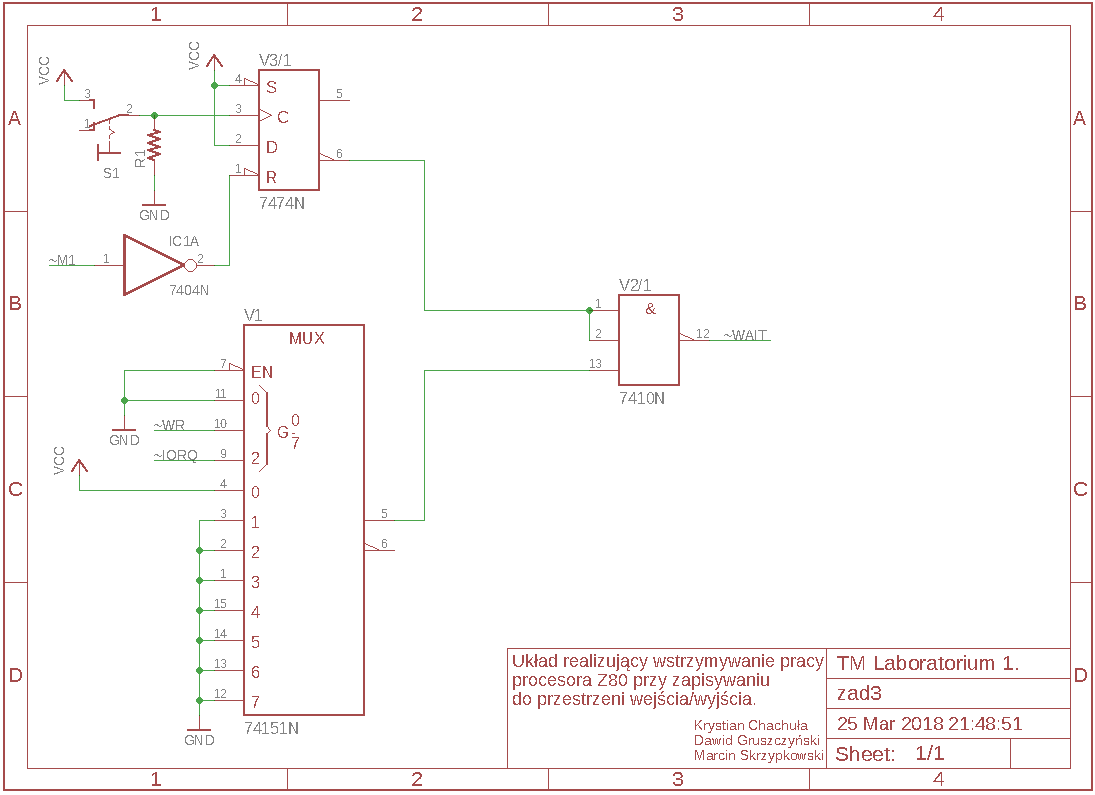
\includegraphics[width=0.75\textwidth]{img/z3.png}
	\caption{Schemat elektryczny układu będącego rozwiązaniem zadania trzeciego}
	\label{fig:z3}
\end{figure}

Układ multipleksera pozostawiliśmy bez zmian, natomiast do bramki \textit{NAND}, z której wychodzi sygnał $\overline{WAIT}$, zamiast najmniej znaczącego bitu rejestru z poprzedniego zadania podłączyliśmy wyjście $\overline{Q}$ przerzutnika.

Następnie zmodyfikowaliśmy kod z poprzedniego zadania, tak by było widać, że procesor jest zatrzymywany po każdym wystąpieniu warunku. Procesor wciąż miał być pułapkowany odczytem z przestrzeni wejścia/wyjścia, więc dodaliśmy jedno polecenie IN, aby można było stwierdzić, że pułapkowanie następuje od razu po zwolnieniu z poprzedniego okresu oczekiwania i gdy są spełnione warunki zadania.

Na rysunku $5$. widoczny jest proces wyzwalania procesora ze stanu oczekiwania, wykonanie kilku instrukcji (dokończenie poprzedniej instrukcji \textit{IN}, wykonanie instrukcji \textit{OUT} i \textit{LD} oraz rozpoczęcie kolejnej instrukcji \textit{IN}) i ponowne wejście do stanu oczekiwania w momencie odczytu z przestrzeni wejścia/wyjścia. Rysunek $6$. pokazuje analogiczną sytuację, z tym że w tym przypadku po wyjściu z pułapki zamiast instrukcji \textit{OUT} i \textit{LD} wykonywana jest instrukcja \textit{JR}.
Wyraźnie widać, że procesor pułapkowany jest z każdym wykryciem instrukcji odczytu z przestrzeni wejścia/wyjścia, można również zidentyfikować, które polecenie wprowadziło procesor do tego stanu. Rysunek piąty przedstawia pułapkowanie w linii programu [\textit{IN A, (04h)}], rysunek 6 w linii programu [\textit{IN A, (0h)}].

Program, który wykorzystaliśmy do testowania zadania 3:

\lstinputlisting{src/2.lst}

\begin{figure}[H]
	\centering
	\begin{subfigure}[H]{0.49\textwidth}
		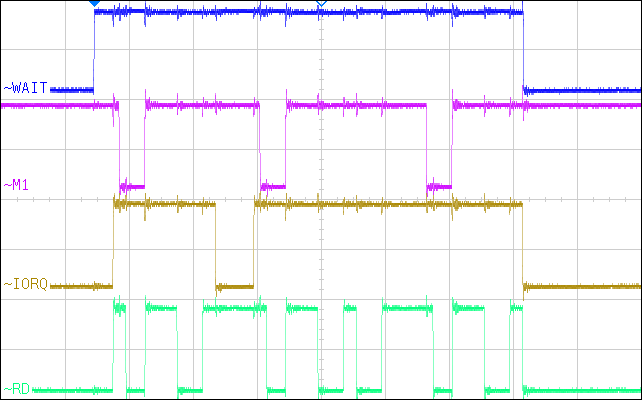
\includegraphics[width=\textwidth]{img/3b.png}
		\caption{Program wstrzymany podczas wykonywania instrukcji \textit{IN A, (0h)} został wznowiony poprzez przełączenie przełącznika, a następnie znów wstrzymany podczas wykonywania instrukcji \textit{IN A, (04h)}}
		\label{fig:3b}
	\end{subfigure}
	\hfill
	\centering
	\begin{subfigure}[H]{0.49\textwidth}
		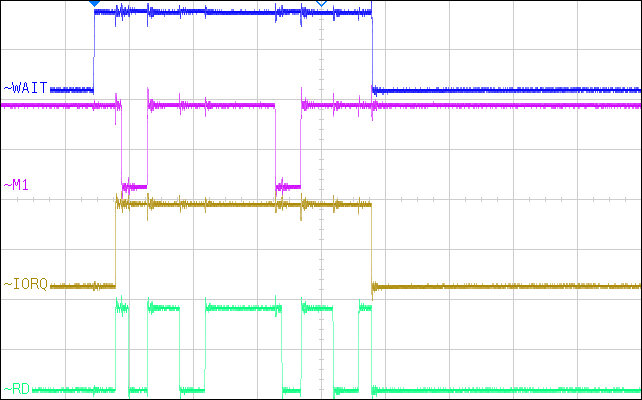
\includegraphics[width=\textwidth]{img/3c.png}
		\caption{Program wstrzymany podczas wykonywania instrukcji \textit{IN A, (04h)} został wznowiony poprzez przełączenie przełącznika, a następnie znów wstrzymany podczas wykonywania instrukcji \textit{IN A, (0h)}}
		\label{fig:3c}
	\end{subfigure}
	\caption{Sygnały sterujące szyną podczas działania układu pułapkującego}
\end{figure}

\section{Problemy}

Podczas prób budowy zaprojektowanych układów natrafiliśmy na kilka problemów, które ostatecznie udało nam się rozwiązać.

Jednym z nich były szybko zanikające sygnały. Spowodowane było to podłączeniem dwóch modułów BNC. Pomimo uzyskania prawidłowego działania układu sygnał $\overline{WAIT}$ był zbyt słaby, aby procesor mógł zauważyć jego zmiany - przez cały czas traktowany był jako sygnał niski. Aby uniknąć tej sytuacji podczas badania układu korzystaliśmy z sond dołączonych do oscyloskopu.

Kolejnym problemem było podłączenie licznika do układu z zadania drugiego. Podczas testów okazało się, że sygnał przeniesienia (sygnał doliczenia do odpowiedniej wartości) znikał zbyt szybko, przez co procesor nie zauważał zmiany generowanego przez nas sygnału $\overline{WAIT}$ i nie zmieniał stanu wyjść. Skutkiem tego, po wyzerowaniu licznika generowany był ponownie sygnał oczekiwania, co powodowało trwałe zatrzymywanie procesora. Problem ten występował przy zliczaniu do 16. Znaleźliśmy dwa rozwiązania tego problemu, jednym było zliczanie do 8 i wykorzystanie najstarszego bitu jako bit przeniesienia, natomiast drugim było użycie rejestru. Ostatecznie zdecydowaliśmy się na wybór drugiej opcji.

\end{document}
